\chapter{MARCO METODOLÓGICO}
\label{cap:metodo}

Este capítulo explica el procedimiento del proyecto con el detalle necesario
para repetirlo. Primero presenta el diagrama de flujo general, el hardware y el
repositorio donde está el código. Después describe cada unidad de trabajo: qué
se ejecuta, con qué entrada y qué salida produce. Las unidades se descomponen en
pasos numerados, y ese es el único contenido del capítulo: aquí no se reporta
ningún valor medido. El Capítulo~\ref{cap:resultados} tiene la misma estructura:
cada sección 3.$x$ de este capítulo tiene su resultado en la sección 4.$x$, con
los mismos títulos y los mismos pasos, de modo que cada paso del método se
comprueba con la salida que produjo.

% =====================================================================
\FloatBarrier
\section{Diagrama de Flujo General}
\label{sec:diagrama-flujo}

La Figura~\ref{fig:flujo} muestra las etapas del proyecto en el orden en que se
ejecutan, de E0 a E5. La letra E indica etapa, para distinguirlas de los pasos
internos de cada módulo, que se numeran Paso~1, Paso~2 y siguientes en las
secciones de cada unidad. Las secciones se procesan una a una, y en cada sección
la etapa de agrupamiento se repite con diez semillas
(Sección~\ref{sec:repeticiones}); el entrenamiento de M2 se realizó una vez.

\begin{figure}[!htbp]
\centering\setstretch{1}
\begin{tikzpicture}[
  font=\scriptsize,
  et/.style={align=center, text width=3.2cm, anchor=north},
  logo/.style={inner sep=0pt},
  fl/.style={-{Latex[length=1.8mm]}, thick},
  bucle/.style={-{Latex[length=1.6mm]}, thick, dashed, black!60},
  vb/.style={font=\tiny, text=black!70}
]
% Fila 1, de izquierda a derecha: E0, E1, E2
\node[logo] (i0) at (0,0)
  {\adjustbox{trim=0 0 {.6667\width} {.12\height}, clip, height=2.5cm}{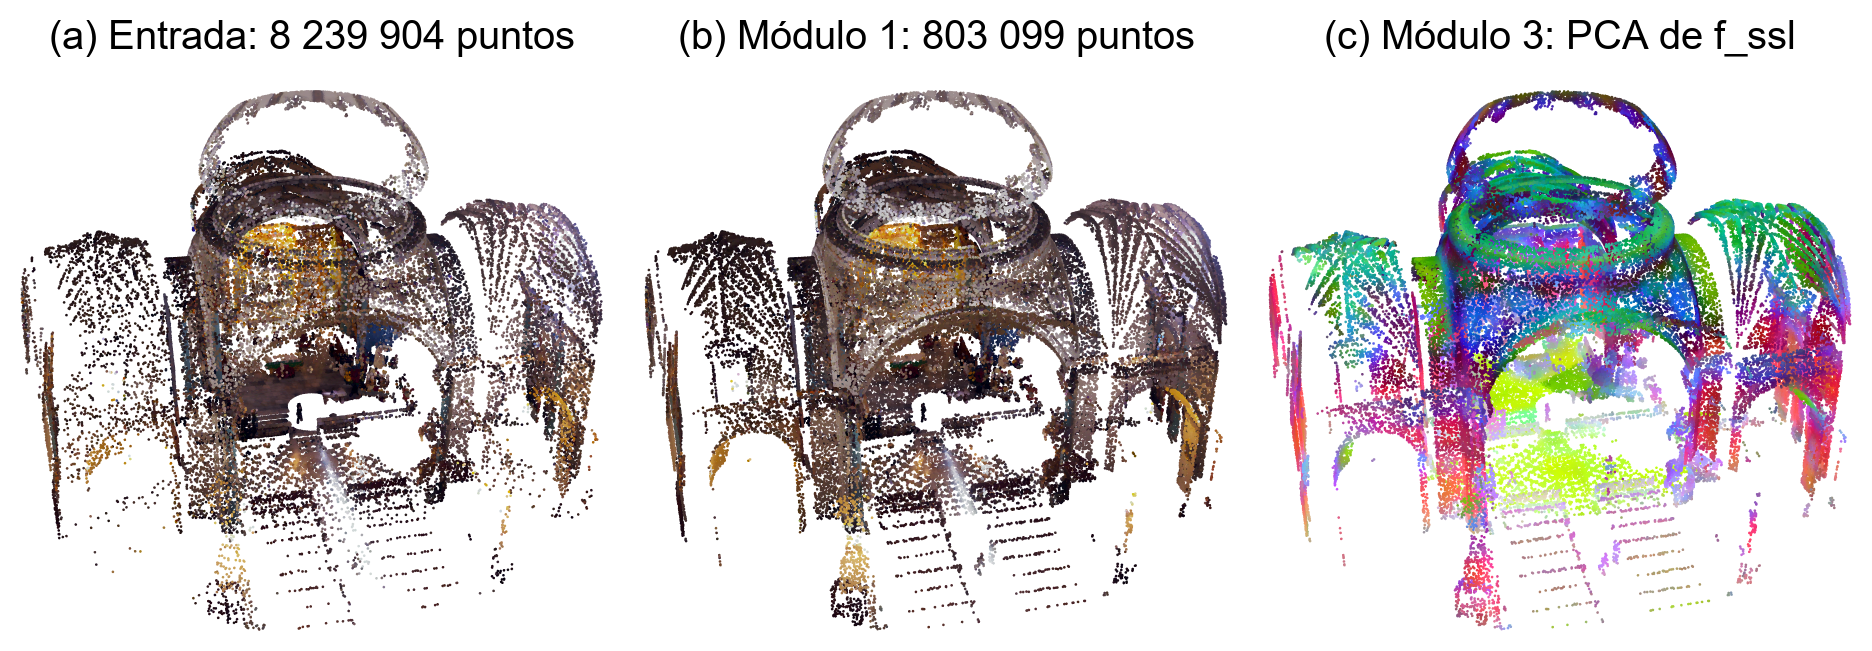
\includegraphics{imagenes/visor_pl13_entrada_m1_m3.png}}\hspace{1mm}
\includegraphics[height=0.8cm]{imagenes/logos/open3d.png}};
\node[et, text width=3.6cm] at (0,-1.7) {\textbf{E0.} 23 archivos LAS: SOR, vóxel y normales, matriz $S$};
\node[logo] (i1) at (5.2,0)
  {\adjustbox{trim={.34\width} 0 {.33\width} 0, clip, height=2.5cm}{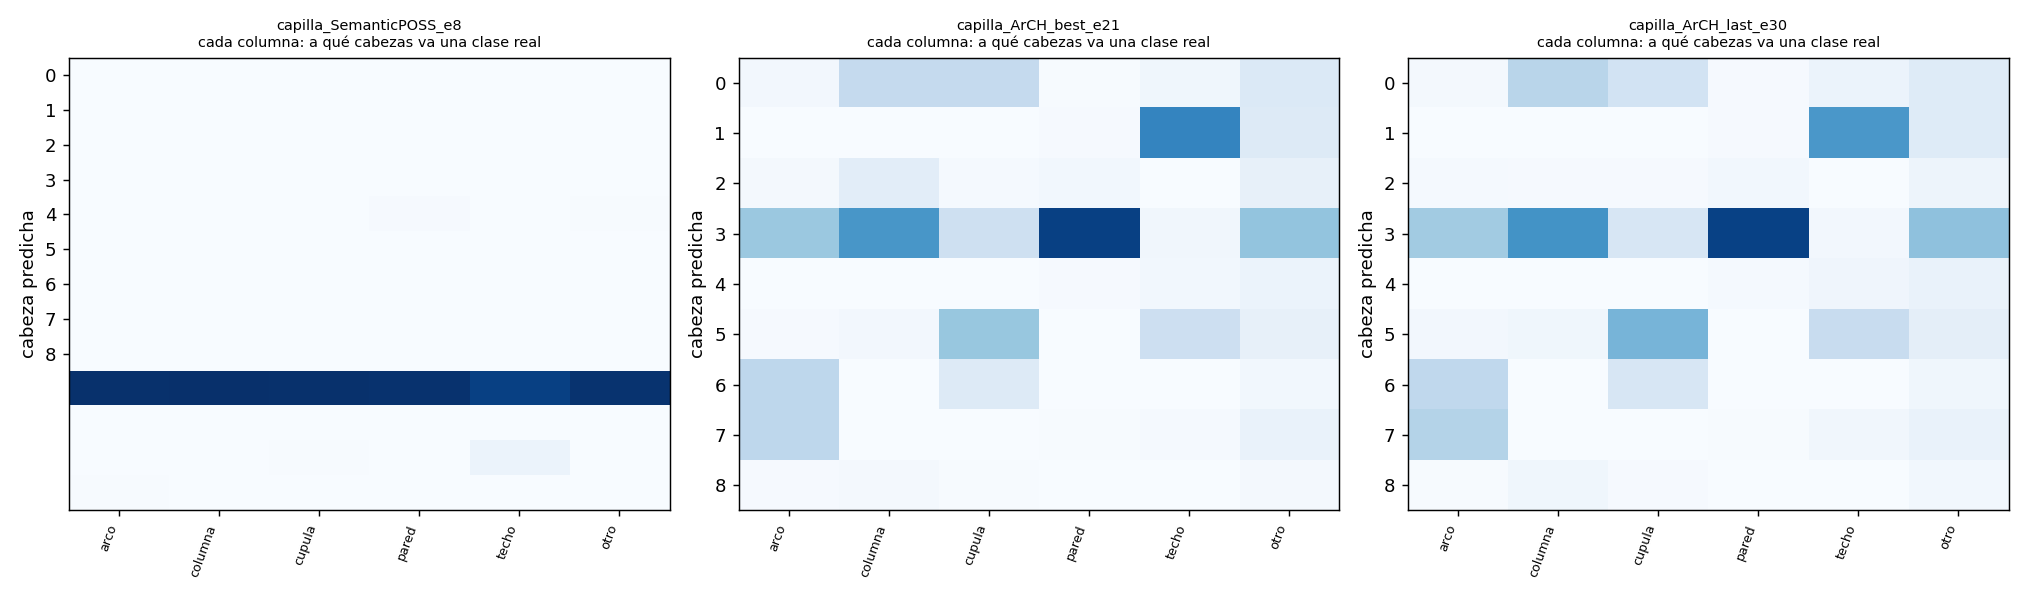
\includegraphics{imagenes/m2_cabeza_x_clase.png}}};
\node[et, text width=3.6cm] at (5.2,-1.7) {\textbf{E1.} Diagnóstico de dominio: M2 de SemanticPOSS en la capilla};
\node[logo] (i2) at (10.4,0)
  {\adjustbox{trim={.34\width} 0 {.33\width} 0, clip, height=2.5cm}{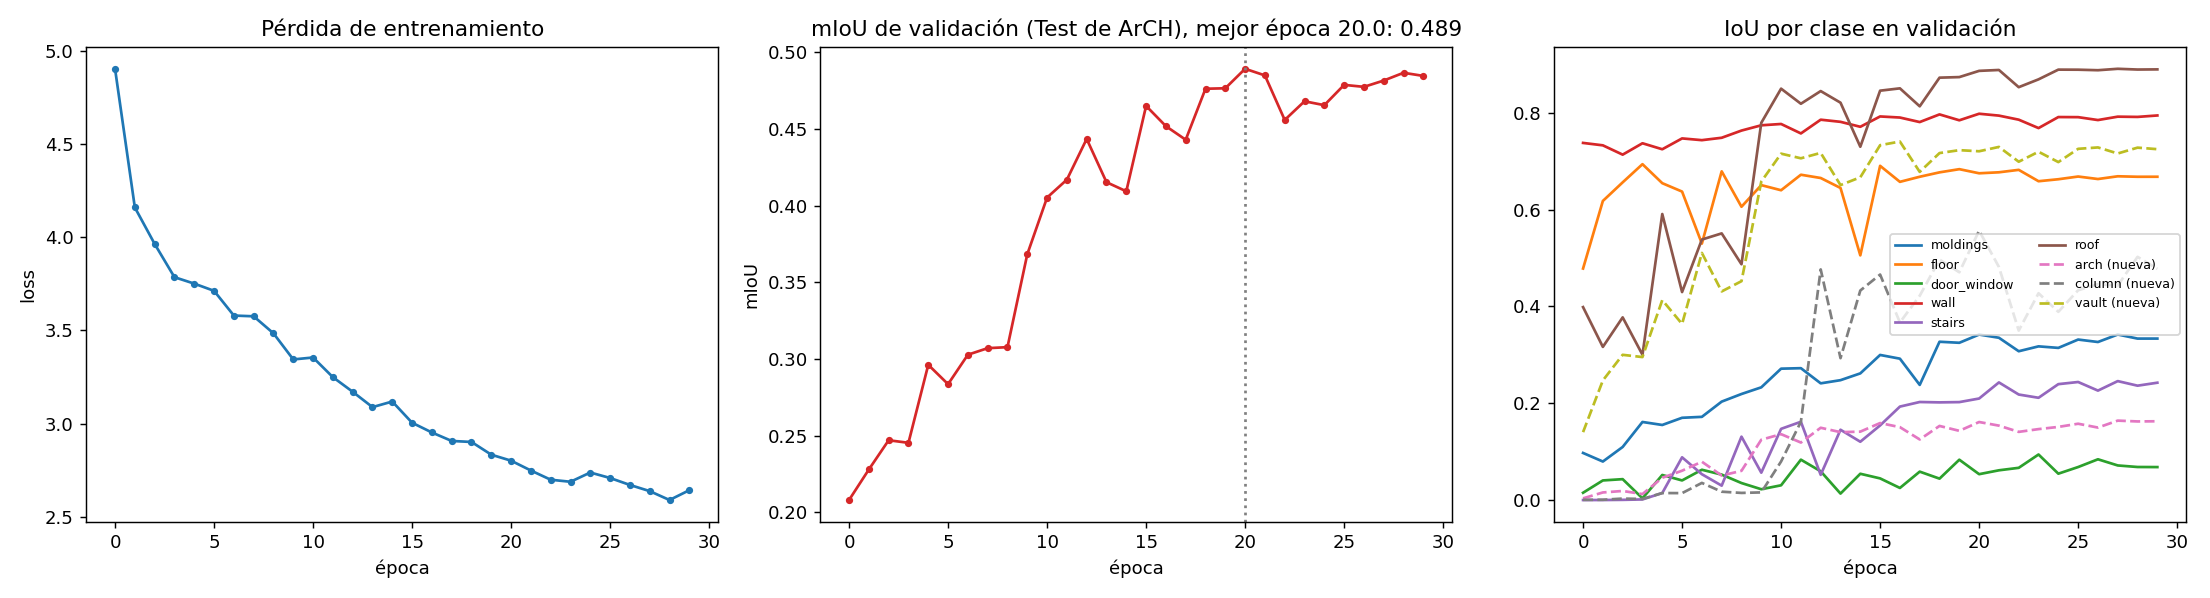
\includegraphics{imagenes/m2_arch_curvas.png}}};
\node[et, text width=3.6cm] (e2) at (10.4,-1.7) {\textbf{E2.} Entrenamiento de M2 con ArCH, una corrida};
% Fila 2, de derecha a izquierda: E3, E4, E5
\node[logo] (i3) at (10.4,-5.0) {\begin{tikzpicture}
  \draw[thick, fill=black!6] (0,0) -- (0,1.4) -- (0.75,1.4) -- (1.1,1.05) -- (1.1,0) -- cycle;
  \draw[thick] (0.75,1.4) -- (0.75,1.05) -- (1.1,1.05);
  \node[font=\scriptsize\ttfamily] at (0.55,0.5) {.npz};
\end{tikzpicture}\hspace{2mm}
\includegraphics[height=1cm]{imagenes/logos/pytorch.png}};
\node[et, text width=3.6cm] at (10.4,-6.4) {\textbf{E3.} Inferencia congelada: $f_{\mathrm{sem}}$ y $f_{\mathrm{ssl}}$ a disco};
\node[logo] (i4) at (5.2,-5.0)
  {\adjustbox{max width=4.4cm, max height=2.5cm}{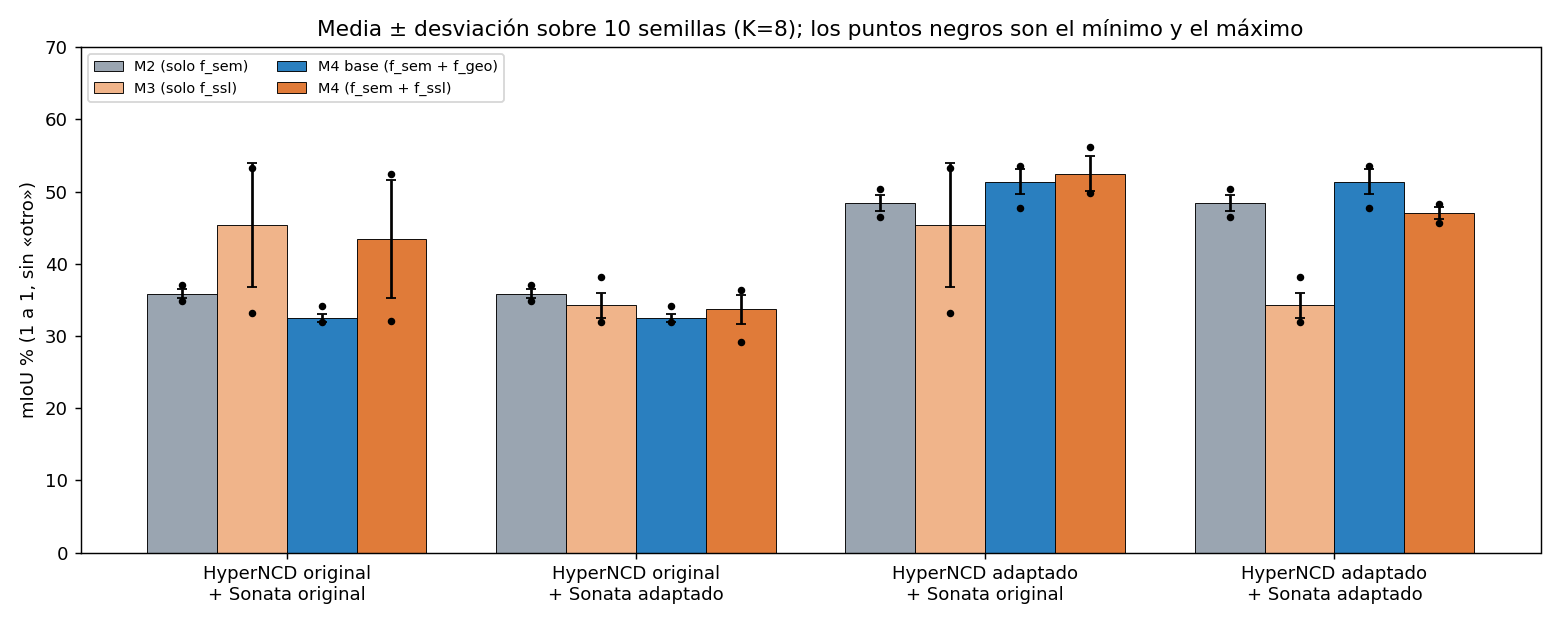
\includegraphics{imagenes/m4_semillas.png}}};
\node[et, text width=3.6cm] (e4) at (5.2,-6.4) {\textbf{E4.} Fusión y agrupamiento M2--M4, $K=8$, $\times10$ semillas};
\node[logo] (i5) at (0,-5.0)
  {\adjustbox{trim=0 0 {.5\width} 0, clip, height=2.5cm}{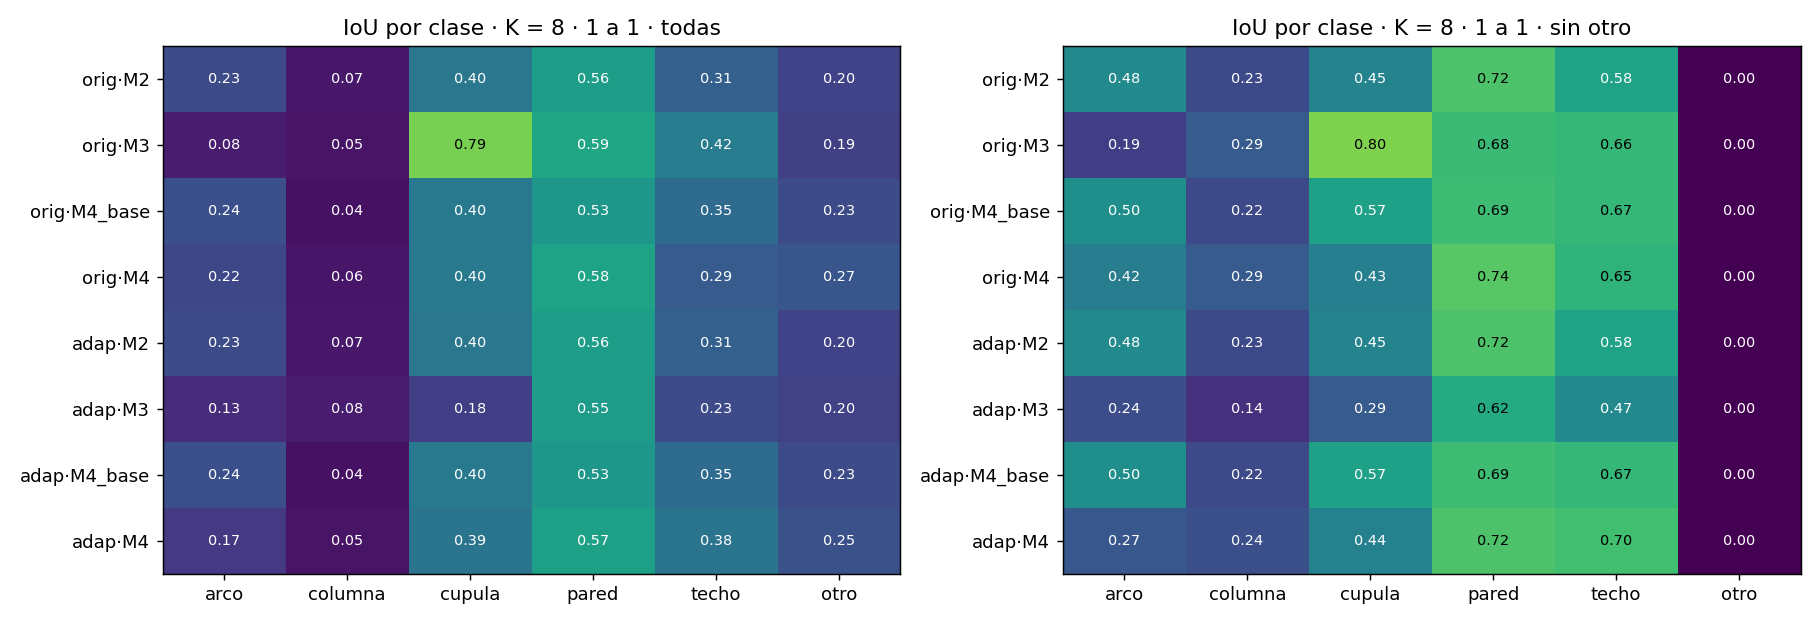
\includegraphics{imagenes/m4_iou_por_clase.png}}};
\node[et, text width=3.6cm] at (0,-6.4) {\textbf{E5.} Evaluación: mIoU uno a uno, NMI, ARI e IoU por clase};
% Flujo
\draw[fl] (i0) -- (i1);
\draw[fl] (i1) -- (i2);
\draw[fl] (i2.south) -- (i3.north);
\draw[fl] (i3) -- (i4);
\draw[fl] (i4) -- (i5);
\end{tikzpicture}
\caption[Flujo general del proyecto]{Flujo general del proyecto. Las imágenes provienen de los resultados del Capítulo~\ref{cap:resultados}. Elaboración propia.}
\label{fig:flujo}
\end{figure}

El flujo añade a la arquitectura la frontera de disco, que exige CUDA 12.4 para
PTv3 y 11.8 para MinkowskiEngine, la asimetría de frecuencia entre el
entrenamiento, la extracción y la fusión, y el bucle de diez semillas
(Sección~\ref{sec:contrato}).

% =====================================================================
\FloatBarrier
\section{Hardware y Repositorio}
\label{sec:hardware-repo}

\paragraph*{Hardware}
El preprocesamiento y la extracción de Sonata se ejecutan en el clúster Khipu de
UTEC; el entrenamiento y la extracción de M2 y la evaluación final, en Google
Colab. Cada paso pide solo lo que necesita. Los recursos del clúster están en la
Tabla~\ref{tab:hardware} y las versiones del entorno en el
\hyperref[sec:anexo-software]{Anexo~A}; el equipo, el tiempo y la memoria de cada
etapa, en la Sección~\ref{sec:res-hardware}.

\paragraph*{Repositorio}
Todo el código está en el repositorio del
proyecto.\footnote{\url{https://github.com/manyorycuevamendoza/PFC1-HyperNCD-Sonata}}
Sus archivos principales están en la Tabla~\ref{tab:archivos}. Los archivos LAS y
las salidas no se guardan en él, y los pesos de Sonata se descargan de
\texttt{facebook/sonata} en Hugging
Face.\footnote{\url{https://huggingface.co/facebook/sonata}}

% =====================================================================
\FloatBarrier
\section{Diseño General del Sistema}
\label{sec:diseno}

El diseño del sistema y el significado de cada módulo, de cada fórmula y de
cada parámetro se describen en la Sección~\ref{sec:diseno-teorico} y se resumen
en la Figura~\ref{fig:diseno}. Esta sección
no repite esa descripción. Fija las propiedades de ejecución que el diagrama no
expresa, es decir, qué corre en paralelo, con qué frecuencia y con qué formato
de intercambio.

Las dos ramas están en paralelo porque ninguna consume la salida de la otra:
parten de la misma nube preparada y solo se encuentran en el Módulo~4. Esa
independencia permite ejecutar el Módulo~3 una sola vez, guardar su salida y
reutilizarla en todas las repeticiones de la fusión.

Las herramientas, el módulo en que interviene cada una y los entornos con sus
versiones se recogen en la Tabla~\ref{tab:herramientas} del \hyperref[sec:anexo-software]{Anexo~A}.

\FloatBarrier
\subsection{Estructura y Contrato de los Módulos}
\label{sec:contrato}

Cada conexión entre módulos transporta un objeto con una forma determinada. La
Tabla~\ref{tab:contrato} declara ese contrato para que cualquier
incompatibilidad de dimensión o de resolución aparezca antes de implementar.

\begin{table}[!htbp]
\centering
\setstretch{1}\small
\setlength{\tabcolsep}{4pt}
\caption[Contrato de los módulos]{Contrato de los módulos. Elaboración propia.}
\label{tab:contrato}
\begin{tabularx}{\linewidth}{@{}l>{\raggedright\arraybackslash}X>{\raggedright\arraybackslash}X>{\raggedright\arraybackslash}p{1.9cm}>{\raggedright\arraybackslash}p{2.0cm}@{}}
\toprule
\textbf{Módulo} & \textbf{Entrada} & \textbf{Salida} & \textbf{Régimen} & \textbf{Frecuencia} \\
\midrule
1 & Archivos LAS de la sección, $N$ puntos & Matriz $S$ de 9 columnas: coord., color, normal & Sin modelo & Una vez por sección \\
2 & Coordenadas de $S$, con característica constante 1 & $f_{\mathrm{sem}}$, 96 dim.\ por punto, rejilla dispersa de 5\,cm & Entrenado antes y aplicado congelado & Entrenamiento una vez; extracción una vez por escena \\
3 & $S$, 9 columnas & $f_{\mathrm{ssl}}$, 1088 dim.\ por punto, rejilla propia de 2\,cm, con índice inverso & Congelado & Una vez por sección \\
4 & $f_{\mathrm{sem}}$ y $f_{\mathrm{ssl}}$ alineados & Prototipos, hipergrafo y pseudo-etiquetas & Fusión posterior, sin gradientes & Una vez por semilla \\
5 & Pseudo-etiquetas y verdad de terreno & Etiqueta por punto, mIoU por clase e interfaz de consulta & Evaluación y consulta & Por corrida \\
\bottomrule
\end{tabularx}
\end{table}

Las salidas de los Módulos~2 y~3 no viven en la misma rejilla. Se concilian con
el índice inverso (Sección~\ref{sec:gridsample}), que se almacena junto con las
características para que el Módulo~4 reciba los dos descriptores alineados punto
a punto.

% Estilos de los diagramas de flujo de los pasos largos.
\tikzset{
  fdato/.style={draw, trapezium, trapezium left angle=72, trapezium right angle=108,
                fill=orange!18, text width=5.6cm, minimum height=0.7cm, align=center,
                inner sep=2pt},
  fop/.style={draw, rounded corners, fill=blue!12, text width=6.2cm,
              minimum height=0.7cm, align=center, inner sep=2pt},
  fdec/.style={draw, diamond, aspect=2.6, fill=yellow!20, text width=2.6cm,
               align=center, inner sep=0pt},
  ffl/.style={-{Latex[length=1.6mm]}, thick},
  fno/.style={draw, rounded corners, fill=red!12, text width=1.9cm,
              minimum height=0.7cm, align=center, inner sep=2pt}
}

\FloatBarrier
\subsection{Visor 3D del Proyecto}
\label{sec:visor}

Para revisar las nubes en cada etapa se construyó un visor propio, el programa
\texttt{visor\_3d.py} de la carpeta \texttt{experimentacion} del repositorio.
Recibe un escaneo en sus distintas etapas y genera una página web que se abre en
el navegador sin instalar nada. La página tiene una sola escena 3D y un botón por
etapa. Las etapas son la entrada cruda, los puntos que descarta el filtrado, la
matriz $S$ de la Unidad~1 con su color y con sus normales, y los descriptores de
Sonata vistos de tres formas. Todas las etapas comparten las coordenadas, la
escala y la cámara. Al cambiar de botón el ángulo no se mueve, así que las etapas
se comparan desde el mismo punto de vista. La página permite girar, acercar y
exportar la vista a PNG. El visor también puede recortar un cubo y dibujar todos
sus puntos.

El visor también comprueba, antes de dibujar, que los descriptores correspondan
a la matriz $S$ (\enlace{sec:u1-reproducibilidad}{verificación de la Unidad~1}).

% =====================================================================
\FloatBarrier
\section{Unidad 1. Preprocesamiento}
\label{sec:unidad1}

La primera unidad convierte un escaneo en bruto, en formato LAS, en la matriz
$S$ que entra a los modelos de la Unidad~2. Corresponde al Módulo~1, descrito en
la Sección~\ref{sec:modulo1}, y está en el programa \texttt{preprocesar.py} del
repositorio. Esta sección describe el procedimiento; su ejecución sobre dos
escaneos reales se presenta en la Sección~\ref{sec:res-unidad1}.

\FloatBarrier
\subsection{Datos de Entrada y Ejecución}
\label{sec:u1-datos}

\paragraph*{El levantamiento.}
La Catedral de Lima se recibe como 23 archivos LAS, que suman 20{,}05\,GB y
589\,708\,290 puntos. Cada archivo es un escaneo de terreno independiente y
trae, por punto, coordenadas UTM, color de 16 bits, intensidad, número de retorno
y clase, de los cuales solo se usan la posición y el color
(Sección~\ref{sec:las}). Por término medio un archivo tiene unos 25{,}6 millones
de puntos y ocupa unos 0{,}87\,GB. Los archivos no traen etiquetas.

\paragraph*{Cómo entran los archivos.}
La unidad de trabajo es la sección (Sección~\ref{sec:seccion}). El programa
\texttt{preprocesar.py} acepta uno o varios archivos LAS en \texttt{--input} y los
une en una sola sección. En el levantamiento completo se usó un archivo por
sección, de modo que hay 23 secciones y cada una produce su propia pareja de
archivos, la matriz $S$ en \texttt{.npy} y los metadatos en \texttt{.json}. Un
archivo se lee por bloques de cinco millones de puntos, pero la sección completa
se acumula en memoria antes del filtrado, por lo que debe caber en la RAM del
nodo.

\paragraph*{Paralelismo.}
El programa no reparte una sección entre procesos ni lee varios archivos a la
vez. El guion de lanzamiento \texttt{preprocesar.sbatch} recorre los archivos de
uno en uno dentro de un solo trabajo del clúster, con los recursos de la
Sección~\ref{sec:hardware-repo} y un límite de cuatro horas. El único
paralelismo es el interno de las operaciones de Open3D. Si un archivo ya tiene su
\texttt{.npy}, el guion lo salta, de modo que un trabajo interrumpido se retoma
sin repetir lo hecho. Como las secciones son independientes
(Sección~\ref{sec:repeticiones}), también podrían lanzarse como trabajos
separados, uno por archivo.

\paragraph*{Comandos en el clúster.}
Los comandos para lanzar cada paso en Khipu, revisar los descriptores y generar
el visor están en el \hyperref[sec:anexo-software]{Anexo~A}. Cada trabajo escribe su registro en
\texttt{logs/}, con los conteos tras cada paso.

\FloatBarrier
\subsection{Procedimiento}
\label{sec:u1-procedimiento}

El programa recibe un archivo LAS y entrega la matriz $S$. Realiza seis pasos,
en este orden, que resume la Figura~\ref{fig:flujo-u1}. Cada paso se describe a
continuación; su pseudocódigo y sus diagramas de flujo están en el
\hyperref[sec:anexo-pasos]{Anexo~F}.
Los parámetros son tres, el tamaño de vóxel $\ell$, el número de vecinos $q$ y
el umbral del filtrado $\lambda$, con valores por defecto $\ell=5$\,cm, $q=20$ y
$\lambda=2$.

\begin{figure}[!htbp]
\centering
\begin{tikzpicture}[
  font=\scriptsize, node distance=3mm,
  caja/.style={draw, rounded corners, text width=5.6cm, minimum height=0.75cm,
               align=center, inner sep=2pt},
  dat/.style={caja, trapezium, trapezium left angle=75, trapezium right angle=105,
               trapezium stretches body, rounded corners=0pt, text width=5.0cm,
               minimum width=6.0cm, fill=orange!18},
  paso/.style={caja, fill=blue!12},
  fl/.style={-{Latex[length=1.8mm]}, thick}
]
\node[dat] (a) {\textbf{Entrada.} Archivo LAS de $N$ puntos};
\node[paso, below=of a] (b) {\textbf{Pasos 1 y 2.} Carga por bloques y centrado};
\node[paso, below=of b] (c) {\textbf{Paso 3.} Filtrado SOR, con $q$ y $\lambda$};
\node[paso, below=of c] (d) {\textbf{Paso 4.} Voxelización al lado $\ell$};
\node[paso, below=of d] (e) {\textbf{Paso 5.} Normales con $q$ vecinos};
\node[dat, below=of e] (f) {\textbf{Paso 6. Salida.} Matriz $S$ y metadatos};
\foreach \u/\v in {a/b, b/c, c/d, d/e, e/f} \draw[fl] (\u) -- (\v);
\end{tikzpicture}
\caption[Flujo del preprocesamiento]{Flujo del preprocesamiento. Elaboración propia.}
\label{fig:flujo-u1}
\end{figure}

\FloatBarrier
\subsubsection*{Paso 1. Carga}
\phantomsection\label{sec:u1-p1}

El archivo se abre con \texttt{laspy} y se lee en bloques de cinco millones de
puntos, para no pedir toda la memoria de una vez, como se explica en la
Sección~\ref{sec:las}. De cada punto se conservan solo la posición $(x,y,z)$ y
el color $(R,G,B)$, que son los datos que usan los modelos. La intensidad, el
número de retorno y la clase se descartan. El color viene en 16 bits, con un
máximo de 65\,535, y se divide entre 256 para llevarlo al rango de 0 a 255.


\FloatBarrier
\subsubsection*{Paso 2. Centrado}
\phantomsection\label{sec:u1-p2}

Las coordenadas vienen en metros sobre el mapa, en el sistema UTM, con valores
de cientos de miles y de millones. Con números tan grandes se pierde precisión
al guardarlos en precisión simple, así que a todos los puntos se les resta el
centro de la caja que los contiene, según la Ecuación~\ref{eq:centrado}. La
forma de la nube no cambia, solo se traslada al origen. El centro restado se
guarda en los metadatos para poder devolver cualquier resultado a su posición
real.


\FloatBarrier
\subsubsection*{Paso 3. Filtrado SOR}
\phantomsection\label{sec:u1-p3}

El escaneo trae puntos sueltos que no pertenecen a ninguna superficie. Para cada
punto se mide la distancia media a sus $q$ vecinos más cercanos. Si esa distancia
supera la media de toda la nube en más de $\lambda$ desviaciones estándar, el
punto se descarta, según la Ecuación~\ref{eq:sor}. El filtrado se hace antes de
voxelizar para que esos puntos no se promedien con los válidos. Es el paso más
lento de la unidad, porque la búsqueda de vecinos recorre la nube completa antes
de la reducción del Paso~4. Es también el único que descarta información de forma
irreversible; la prueba que justifica su necesidad y sus dos parámetros está en la
Sección~\ref{sec:param-p1}.


\FloatBarrier
\subsubsection*{Paso 4. Voxelización}
\phantomsection\label{sec:u1-p4}

El escáner mide muchos más puntos cerca de él que lejos. Para igualar la
densidad, el espacio se divide en cubos de lado $\ell$ y los puntos de cada
cubo se sustituyen por uno solo, con su posición y su color promedio, según la
Ecuación~\ref{eq:voxel}. No se pierde ninguna superficie, cambia cuántos puntos
la describen. El vóxel fija también el límite de resolución de la unidad, porque
dos superficies separadas por menos de $\ell$ quedan representadas por los
mismos representantes y dejan de distinguirse.


\FloatBarrier
\subsubsection*{Paso 5. Normales}
\phantomsection\label{sec:u1-p5}

La normal indica hacia dónde mira la superficie en cada punto, y el escáner no
la mide. Se estima con los $q$ vecinos de cada representante, según la
Ecuación~\ref{eq:normal}. La dirección en la que esos vecinos menos se dispersan
es la perpendicular a la superficie. Todas las normales se orientan con
$n_z\geq 0$ para que sean consistentes entre sí. La estimación depende de que
los $q$ vecinos describan bien la superficie local, condición que no se cumple en
las zonas ralas, lejos del escáner.


\FloatBarrier
\subsubsection*{Paso 6. Escritura}
\phantomsection\label{sec:u1-p6}

Se guarda la matriz $S$, descrita en la Ecuación~\ref{eq:sj}, con una fila por
representante y sus nueve valores, la posición, el color y la normal, en
precisión simple. Junto a ella se escribe un archivo de metadatos en
\texttt{.json} con ocho campos: \texttt{voxel}, el lado del vóxel en metros;
\texttt{q}, los vecinos del filtrado y de las normales; \texttt{lambda}, el
umbral del filtrado; \texttt{offset\_utm}, el centro restado en el Paso~2;
\texttt{n\_crudo}, \texttt{n\_sor} y \texttt{n\_voxel}, los puntos que quedan
tras la carga, tras el filtrado y tras la voxelización; y \texttt{segundos}, el
tiempo total.


\FloatBarrier
\subsection{Verificación y Reproducibilidad}
\label{sec:u1-reproducibilidad}

El programa no tiene pasos aleatorios, de modo que la misma entrada produce la
misma salida. Se ejecuta con una orden como la siguiente, con los valores por
defecto del programa.
\begin{lstlisting}[style=comando]
python preprocesar.py --input PL13_SCN0001.las \
       --output PL13_SCN0001_preprocesado \
       --voxel 0.05 --q 20 --lam 2
\end{lstlisting}
El programa tiene además dos opciones que no cambian el procedimiento descrito:
\texttt{--chunk}, el tamaño de bloque del Paso~1, con valor por defecto
$5\times10^{6}$, y \texttt{--prevoxel}, un vóxel previo al filtrado para nubes
muy densas, desactivado por defecto (valor 0) y no usado en este proyecto.
Una repetición se comprueba comparando los conteos del archivo de metadatos,
\texttt{n\_crudo}, \texttt{n\_sor} y \texttt{n\_voxel}, con los de la corrida de
referencia. Deben coincidir exactamente.

Lo que se repite son los puntos, no su orden de filas. Como los descriptores de
Sonata se asocian a los puntos por ese orden, cada archivo de descriptores debe
usarse con la misma matriz $S$ que entró a Sonata, y no con otra repetición del
preprocesamiento. El visor de la Sección~\ref{sec:visor} comprueba esa
correspondencia antes de dibujar y se detiene con un aviso si no se cumple.



% =====================================================================
\FloatBarrier
\section{Unidad 2. Extracción de Descriptores y Fusión}
\label{sec:unidad2}

La segunda unidad abarca los Módulos~2, 3 y~4. Las dos ramas de extracción
producen, sobre la misma sección preparada, los dos descriptores que el punto de
fusión concatena.

\FloatBarrier
\subsection{Rama Semántica}
\label{sec:rama-sem}

La rama semántica es el Módulo~2 (Sección~\ref{sec:modulo2}). Es un módulo
entrenable, pero en el flujo aplicado a la Catedral se separan dos fases. Primero
se entrena HyperNCD con un conjunto etiquetado; después se carga el checkpoint en
modo de evaluación y se extrae $f_{\mathrm{sem}}$ una sola vez por escena. El
programa \texttt{predecir\_hyperncd.py} cuantiza XYZ a 5\,cm, asigna la
característica constante 1, ejecuta MinkowskiUNet-34C sin gradiente y guarda el
descriptor de 96 dimensiones, las cabezas y el índice inverso.

Se comparan dos entrenamientos. El primero usa SemanticPOSS, con nueve clases
conocidas y cuatro novedosas en la partición~0. El segundo usa ArCH
\cite{matrone2020benchmark}: se ignora \emph{other}; son conocidas molduras,
piso, puerta/ventana, pared, escalera y cubierta, y novedosas arco, columna y
bóveda. Sus 15 escenarios de entrenamiento y dos de prueba se voxelizan a
5\,cm y se dividen en bloques de 10\,m. Cada muestra toma hasta 60\,000 puntos y
las regiones novedosas usan DBSCAN de radio 0,5\,m. Las escenas oficiales de
prueba se usan como validación para seleccionar el checkpoint; su mIoU no se
considera una prueba externa independiente.

\FloatBarrier
\subsection{Rama Auto-supervisada Congelada}
\label{sec:rama-ssl}

La rama auto-supervisada corresponde al Módulo~3 (Sección~\ref{sec:modulo3}) y
está en el programa \texttt{extraer\_features.py} del repositorio. Se ejecuta una
sola vez por sección y su salida se escribe en disco para reutilizarla en todas
las épocas. Recibe la matriz $S$ que entrega la Unidad~1 y entrega un archivo
\texttt{.npz} con los descriptores. Realiza cinco pasos, que resume la
Figura~\ref{fig:flujo-sonata}. Cada paso se describe a continuación; su pseudocódigo y sus diagramas de
flujo están en el \hyperref[sec:anexo-pasos]{Anexo~F}.

\begin{figure}[!htbp]
\centering
\begin{tikzpicture}[
  font=\scriptsize, node distance=3mm,
  caja/.style={draw, rounded corners, text width=5.6cm, minimum height=0.75cm,
               align=center, inner sep=2pt},
  dat/.style={caja, trapezium, trapezium left angle=75, trapezium right angle=105,
               trapezium stretches body, rounded corners=0pt, text width=5.0cm,
               minimum width=6.0cm, fill=orange!18},
  paso/.style={caja, fill=blue!12},
  cong/.style={caja, fill=purple!14},
  fl/.style={-{Latex[length=1.8mm]}, thick}
]
\node[dat] (a) {\textbf{Entrada.} Matriz $S$ de la sección};
\node[paso, below=of a] (b) {\textbf{Pasos 1 y 2.} Carga de $S$ y de los pesos};
\node[paso, below=of b] (c) {\textbf{Paso 3.} Centrado y rejilla de lado $g$};
\node[cong, below=of c] (d) {\textbf{Paso 4.} Codificador PTv3 congelado};
\node[dat, below=of d] (e) {\textbf{Paso 5. Salida.} Archivo \texttt{.npz} con $f_{\mathrm{ssl}}$};
\foreach \u/\v in {a/b, b/c, c/d, d/e} \draw[fl] (\u) -- (\v);
\end{tikzpicture}
\caption[Flujo de la extracción con Sonata]{Flujo de la extracción con Sonata. Elaboración propia.}
\label{fig:flujo-sonata}
\end{figure}

\FloatBarrier
\subsubsection*{Paso 1. Carga de la matriz}
\phantomsection\label{sec:u2-p1}

El programa lee la matriz $S$ que dejó la Unidad~1 y la separa en tres partes,
la posición, el color y la normal. Son las tres entradas que espera Sonata. La
matriz se lee completa porque, tras la voxelización, ya cabe en memoria.


\FloatBarrier
\subsubsection*{Paso 2. Carga del modelo}
\phantomsection\label{sec:u2-p2}

El programa carga los pesos públicos de Sonata, del repositorio
\texttt{facebook/sonata} indicado en la Sección~\ref{sec:hardware-repo}. Se
descargan una sola vez, desde
el nodo de acceso del clúster, y quedan guardados en disco, porque los nodos con
GPU no tienen salida a internet. El modelo se pasa a la GPU en modo de
inferencia, de modo que sus pesos no cambian. FlashAttention se desactiva porque
no está instalada en el clúster, y el tamaño de parche del codificador se fija
en 1024 puntos.


\FloatBarrier
\subsubsection*{Paso 3. Preparación}
\phantomsection\label{sec:u2-p3}

El programa aplica la rutina de preparación de Sonata. Primero traslada la nube,
de modo que el centro de la caja en $x$ e $y$ y el punto más bajo en $z$ quedan
en el origen. Después la muestrea con una rejilla de lado $g$, según la
Sección~\ref{sec:gridsample}, conservando un punto elegido al azar por celda, y
guarda un índice inverso que dice a qué celda pertenece cada punto de entrada.
Ese índice permite devolver más adelante los descriptores a cada punto de $S$
(Ec.~\eqref{eq:upcast}). Por último divide el color entre 255. El lado de la
rejilla es una opción del programa, \texttt{--grid}, con valor por defecto
$g=2$\,cm, el mismo con que se preentrenó Sonata.


\FloatBarrier
\subsubsection*{Paso 4. Inferencia}
\phantomsection\label{sec:u2-p4}

El programa pasa la nube preparada por el codificador PTv3 de Sonata, sin
calcular gradientes. Las operaciones y sus fórmulas están en la
Sección~\ref{sec:codificador-ptv3}, y el detalle de cada etapa en el \hyperref[sec:arq-sonata]{Anexo~C}.
La inferencia tiene cuatro subpasos, que resume la Figura~\ref{fig:m3-inferencia}.
Las cinco etapas tienen 3, 3, 3, 12 y 3 bloques; entre etapas, el
\emph{pooling} lleva la celda de 2 a 4, 8, 16 y 32\,cm y los canales de 48 a 96,
192, 384 y 512.
Dentro de la GPU los parches y las cabezas de atención se calculan a la vez; las
etapas, en cambio, van en orden, porque cada una usa la salida de la anterior.


\FloatBarrier
\subsubsection*{Paso 5. Escritura}
\phantomsection\label{sec:u2-p5}

El programa guarda en un archivo \texttt{.npz} todo lo que necesita la
Unidad~2 para usar los descriptores sin volver a ejecutar Sonata. Son seis
campos: \texttt{feat}, los descriptores $f_{\mathrm{ssl}}$ de 1088 valores por
punto de la rejilla, en precisión media para reducir el tamaño a la mitad;
\texttt{coord}, la posición de cada punto de la rejilla; \texttt{inverse}, la
celda de la rejilla a la que pertenece cada punto de $S$; \texttt{grid\_size},
el lado $g$ de la rejilla; \texttt{n\_original}, el número de puntos de $S$; y
\texttt{semilla}, la semilla del muestreo del Paso~3
(Sección~\ref{sec:param-replicacion}).


\FloatBarrier
\subsubsection*{Observables}
\label{sec:observables}

El diseño declara por adelantado qué debe medir cada corrida de esta rama, de
modo que el resultado se pueda contrastar con lo previsto. Son seis observables:
la dimensión de $f_{\mathrm{ssl}}$, que fija la entrada del Módulo~4 y debe
valer 1088; los puntos retenidos tras el muestreo por rejilla, que determinan el
tamaño del almacenamiento y la resolución efectiva; la VRAM pico, que contrasta
con la cota analítica de 4{,}2\,GB calculada para una sección de
$3\times10^{5}$ puntos; el tiempo de inferencia por sección, que sustituye a la
estimación de costo; el rendimiento en puntos por segundo, que permite
extrapolar a otras secciones; y el tamaño del archivo de descriptores, que
dimensiona el almacenamiento del proyecto. Los valores salen del registro que
imprime \texttt{extraer\_features.py} en la misma corrida, salvo el tamaño del
archivo, que se lee del disco.

Si la memoria crece con el número de puntos, los escaneos más grandes del
levantamiento podrían no caber en una sola pasada. Para ellos se prevé dividir
la sección en bloques espaciales con un margen de solape y procesar cada bloque
por separado.

\subsubsection*{Revisión de los descriptores}
\label{sec:revision-descriptores}

Los descriptores no traen etiquetas, así que su calidad todavía no se puede
medir con una métrica de acierto. Se revisan con el visor
de la Sección~\ref{sec:visor} y se miden con \texttt{visualizar\_features.py}, de la
carpeta \texttt{experimentacion}. Ambos programas aplican el mismo
procedimiento. Restan a los descriptores la media de una muestra de 100\,000
puntos elegidos con semilla 0 y los normalizan a largo 1. Sobre esa base
producen tres vistas. La primera proyecta los 1088 valores de cada punto sobre
sus tres componentes principales y los usa como color, de modo que un mismo
color indica descriptores parecidos. La segunda colorea cada punto según su
similitud coseno con un punto de consulta, marcado con un rombo negro, en rojo
si se parece y en azul si no. La tercera agrupa los descriptores normalizados en
ocho grupos con $k$-means, programado en NumPy, con 30 iteraciones y centros
ajustados sobre esa misma muestra, sin etiquetas.

La medida de acierto es el \emph{linear probing}, descrito en la
Sección~\ref{sec:probing}, que requiere puntos etiquetados. Mientras tanto, la
dispersión de los descriptores se resume con la varianza explicada por las
primeras componentes principales y con el rango efectivo. Las varianzas se
calculan por descomposición en valores singulares de esa muestra y el rango
efectivo es la exponencial de la entropía de las varianzas normalizadas,
$\exp\!\big(-\sum_k p_k\ln p_k\big)$. Vale 1 si todo queda en una sola
dirección, lo que indicaría un colapso, y 1088 si se reparte por igual.



\FloatBarrier
\subsection{Punto de Fusión}
\label{sec:fusion}

El Módulo~4 (Sección~\ref{sec:modulo4}) se ejecutó con la escena de control
(Sección~\ref{sec:res-unidad3}). Concatena los dos descriptores según la
Ec.~\eqref{eq:hibrido} y deja igual todo lo posterior (Ec.~\eqref{eq:afinidad},
$M=8$ vecinos), condición que hace interpretable la ablación. Antes de contar
con datos reales, el módulo se verificó sobre una escena sintética con
descriptores de calidad controlada; esa prueba, sus algoritmos paso a paso y sus
cinco barridos de parámetros se trasladaron al
\hyperref[sec:m4-simulado]{Anexo~D} para evitar redundancia con los resultados
reales. Sus dos lecciones se conservan aquí: el aporte de $f_{\mathrm{ssl}}$
solo aparece cuando la forma no basta para separar las clases, y el desbalance
entre clases novedosas es un modo de fallo del equilibrio de Sinkhorn que debe
vigilarse con la tolerancia $\gamma$.

% =====================================================================
\FloatBarrier
\section{Justificación de los Parámetros del Procedimiento}
\label{sec:parametros}

Cada paso fija algún valor: cuántos vecinos mirar, cuánto mide un vóxel, con
qué precisión guardar un número. Esta sección explica de dónde sale cada valor,
qué aporta cada paso y cómo se comprobará que los valores elegidos son
adecuados. La Tabla~\ref{tab:parametros} resume los valores. Los que dicen
«falta medirlo» se usan hoy por defecto y son los que comprueban las pruebas P0
a P5 de la Sección~\ref{sec:param-criterio}.

\begin{table}[!htbp]
\centering
\setstretch{1}\small
\setlength{\tabcolsep}{4pt}
\caption[Parámetros del procedimiento]{Parámetros del procedimiento, de dónde sale cada valor y qué prueba lo comprueba. Elaboración propia.}
\label{tab:parametros}
\begin{tabularx}{\linewidth}{@{}>{\raggedright\arraybackslash\hsize=0.8\hsize}X>{\raggedright\arraybackslash\hsize=0.65\hsize}X>{\raggedright\arraybackslash\hsize=1.55\hsize}Xl@{}}
\toprule
\textbf{Parámetro} & \textbf{Valor} & \textbf{Por qué este valor} & \textbf{Prueba} \\
\midrule
\multicolumn{4}{@{}l}{\textit{Unidad 1}}\\
Tamaño de bloque (Paso~1) & $5\times10^{6}$ & Solo limita la memoria; no cambia el resultado & P0 \\
Escala del color (Paso~1) & $/256$ & Sonata espera color de 0 a 255 & --- \\
Vecinos $q$ del filtrado (Paso~3) & 20 & Valor por defecto de Open3D; falta medirlo & P1 \\
Umbral $\lambda$ (Paso~3) & 2 & Valor por defecto de Open3D; falta medirlo & P1 \\
Lado del vóxel $\ell$ (Paso~4) & 5\,cm & Valor inicial; falta medirlo & P2 \\
Vecinos de las normales (Paso~5) & 20 & Comparte el $q$ del filtrado; falta medirlo & P3 \\
Precisión de $S$ (Paso~6) & Simple & Solo afecta al tamaño en disco & P4 \\
\midrule
\multicolumn{4}{@{}l}{\textit{Unidad 2}}\\
Tamaño de parche (Paso~2) & 1024 & Valor inicial; falta medirlo & P5 \\
FlashAttention (Paso~2) & No & No está instalada en el clúster & --- \\
Rejilla $g$ (Paso~3) & 2\,cm & Es la de preentrenamiento de Sonata & P2 \\
Etapas del \emph{up-cast} (Paso~4) & 3, 4 y 5 & Las define Sonata & --- \\
Precisión del \texttt{.npz} (Paso~5) & Media & Solo afecta al tamaño en disco & P4 \\
\midrule
\multicolumn{4}{@{}l}{\textit{Módulo 4 y Unidad 3}}\\
$\alpha$, $M$, $\tau$, $\epsilon$, $\epsilon_{\mathrm{sk}}$, $\gamma$ & \hyperref[sec:anexo-nomenclatura]{Anexo~B} & Se calibran en el objetivo OE2 & OE2 \\
\bottomrule
\end{tabularx}
\end{table}

\FloatBarrier
\subsection{Función de Cada Paso y Efecto de Omitirlo}
\label{sec:param-funcion}

Antes de discutir valores hay que justificar que cada paso exista. Los seis pasos
de la Unidad~1 y los cuatro de la rama auto-supervisada hacen un trabajo que los
siguientes necesitan: limitar la memoria, conservar la precisión, retirar puntos
sueltos, igualar la densidad, dar a Sonata su tercera entrada, y escribir una
salida que separe las unidades. La Tabla~\ref{tab:funcion}, en el
\hyperref[sec:anexo-parametros]{Anexo~H}, dice qué aporta cada uno y qué pasaría
sin él.

\FloatBarrier
\subsection{Pruebas de los Parámetros}
\label{sec:param-criterio}
\phantomsection\label{sec:param-p0}\phantomsection\label{sec:param-p1}%
\phantomsection\label{sec:param-p2}\phantomsection\label{sec:param-p3}%
\phantomsection\label{sec:param-p4}\phantomsection\label{sec:param-p5}%

Cada prueba cambia un solo parámetro sobre la misma sección, deja fijos los
demás y mide la salida con cuatro indicadores: la rugosidad, la dispersión
angular de las normales, el ARI y el NMI frente a la configuración de referencia
(Ecs.~\eqref{eq:ari} y~\eqref{eq:nmi}) y el costo. Se elige el valor más barato a
partir del cual los indicadores dejan de mejorar. Las seis pruebas, P0 a P5, están
en la Tabla~\ref{tab:pruebas} del \hyperref[sec:anexo-parametros]{Anexo~H}.

\FloatBarrier
\subsection{Replicación del Procedimiento}
\label{sec:param-replicacion}

El procedimiento de las Unidades~1 y~2 es replicable porque ningún valor está
escondido en el código, porque cada parámetro es una opción de la línea de
órdenes, porque cada corrida deja constancia de lo que hizo en sus metadatos y
porque el código, la instalación y los pesos están en el
\enlace{sec:hardware-repo}{repositorio}. La única fuente de azar es la rutina de
preparación de Sonata, que elige un punto al azar cuando varios caen en la misma
celda; el programa \texttt{extraer\_features.py} fija ahora una semilla, con
valor 0 por defecto, y la guarda en el archivo. Los cinco pasos para replicar una
configuración, la tabla de cambios (Tabla~\ref{tab:replica}) y los límites de la
replicación están en el \hyperref[sec:anexo-parametros]{Anexo~H}.

% =====================================================================
\FloatBarrier
\section{Unidad 3. Entrenamiento, Calibración y Evaluación}
\label{sec:unidad3}

La tercera unidad describe cómo se ejecuta el sistema en el tiempo, con qué
procedimiento se obtienen las mediciones y bajo qué protocolo se repiten.

\FloatBarrier
\subsection{Procedimiento Experimental}
\label{sec:procedimiento}

El procedimiento se organiza en seis pasos reproducibles, correspondientes a los
rótulos E0 a E5 de la Figura~\ref{fig:flujo}. La ejecución final separa el
entrenamiento de HyperNCD, la extracción congelada de ambas ramas y la fusión
posterior, por lo que no existe entrenamiento conjunto HyperNCD--Sonata:

\begin{enumerate}\setlength{\itemsep}{2pt}
\item \textbf{E0. Preparación.} Preprocesamiento de los escaneos de la Catedral
de Lima y construcción de las entradas requeridas por las ramas semántica y
auto-supervisada.
\item \textbf{E1. Diagnóstico de dominio.} Aplicación del checkpoint entrenado
con SemanticPOSS a una sección de la catedral. La concentración de 98,4\,\% de
los puntos en una sola cabeza reveló un desplazamiento de dominio y motivó el
cambio de datos de entrenamiento.
\item \textbf{E2. Entrenamiento de M2.} Entrenamiento desde cero de HyperNCD con
ArCH~\cite{matrone2020benchmark}: 15 escenas de entrenamiento y dos escenas de
prueba utilizadas como validación, seis clases conocidas, tres novedosas y la
clase \emph{other} ignorada en la evaluación principal.
\item \textbf{E3. Inferencia congelada.} Carga del mejor checkpoint de M2 y
extracción, bajo \texttt{eval()} y \texttt{no\_grad()}, de $f_{\mathrm{sem}}$
de 96 dimensiones, logits e índice inverso. En una ejecución independiente se
extrae $f_{\mathrm{ssl}}$ con Sonata. Ninguna rama se reajusta sobre la catedral.
\item \textbf{E4. Fusión posterior.} Lectura de los descriptores almacenados y
comparación de M2, M3, M4 base y M4. La fusión y el agrupamiento operan después
de la inferencia; no retropropagan gradientes hacia HyperNCD ni Sonata.
\item \textbf{E5. Evaluación.} Cómputo de mIoU con emparejamiento uno a uno,
NMI, dominancia de cabezas y estadísticos de las semillas de agrupamiento. Se
reportan por separado las métricas con y sin \emph{other} para evitar que la
clase residual domine la interpretación.
\end{enumerate}

\FloatBarrier
\subsection{Protocolo de Repetición}
\label{sec:repeticiones}

Las secciones son independientes. Ninguna necesita información de otra, de modo
que cada una constituye una medición separada y todas pueden ejecutarse de forma
simultánea.

El entrenamiento de HyperNCD con ArCH se realizó una vez; por ello, el valor de
validación del checkpoint no debe presentarse como media de entrenamientos. La
comparación posterior de M2, M3, M4 base y M4 se repitió con diez semillas del
agrupamiento. Se reportan media y desviación estándar entre esas diez semillas.
Esta dispersión caracteriza la estabilidad del agrupamiento, pero \textbf{no}
equivale a diez reentrenamientos de HyperNCD o Sonata.

Como las secciones son independientes, pueden repartirse entre varias GPU. Con
$n_{\mathrm{gpu}}$ unidades y $n_{\mathrm{sec}}$ secciones, la aceleración frente
a la ejecución secuencial es
\begin{equation}
A=\min\left(n_{\mathrm{gpu}},\,n_{\mathrm{sec}}\right),
\label{eq:aceleracion}
\end{equation}
porque una sección no se reparte entre unidades. Con 23 secciones, más de 23
GPU no acortan el tiempo total.

\FloatBarrier
\subsection{Trazabilidad de la Métrica}
\label{sec:trazabilidad}

La métrica se reporta en dos puntos, con \emph{linear probing} sobre el
descriptor y con mIoU al final, según la atribución por etapas de la
Sección~\ref{sec:metricas-hibrido}.

\FloatBarrier
\subsection{Verificación Empírica del Entorno de Cómputo}
\label{sec:entorno-computo}

Antes de ejecutar el procedimiento fue necesario dejar operativo el entorno de
HyperNCD en el clúster Khipu, porque su repositorio no declara todas sus
dependencias. Lo difícil fue compilar MinkowskiEngine contra CUDA~11.8 con un
compilador GNU compatible. La prueba del entorno consiste en lanzar una
corrida de entrenamiento y comprobar hasta qué etapa llega.

% =====================================================================
\FloatBarrier
\section{Riesgos y Mitigación}
\label{sec:riesgos}

\paragraph*{(i) Disponibilidad de la nube anotada.} NCD exige al menos las clases
conocidas etiquetadas. Se asume la anotación manual de una sección de referencia
con $\geq$4 clases base; si el levantamiento llega sin etiquetas, esa anotación
se vuelve tarea previa del cronograma y condiciona el inicio de OE1.

\paragraph*{(ii) Acceso y configuración del clúster.} La configuración de GPU de
Khipu ha cambiado respecto de la documentada previamente. Por ello el proyecto no
estima tiempos de calendario. Verifica empíricamente el hardware asignado
(Tabla~\ref{tab:hardware}, Sección~\ref{sec:entorno-computo}).

\paragraph*{(iii) Sustitución frente a concatenación (Plan~B).} Si el reemplazo
directo degrada el rendimiento, la variante es concatenar
$F_i=[f_{\mathrm{sem}};f_{\mathrm{geo}};f_{\mathrm{ssl}}]$, dejando que el módulo
de prototipos pondere las tres fuentes. Cualquier resultado, sea mejora, paridad o
degradación, documentado con ablación es reportable.

% =====================================================================
\FloatBarrier
\section{Conclusión del Marco Metodológico}
\label{sec:conclusion-metodo}

Las tres unidades preparan la nube, extraen los dos descriptores y los evalúan
aislando una sola variable, el descriptor que entra al módulo de prototipos. Así,
cualquier diferencia en las métricas del capítulo siguiente se atribuye al
reemplazo de $f_{\mathrm{geo}}$ por $f_{\mathrm{ssl}}$.
